\documentclass[a4paper]{article}

%% Language and font encodings
\usepackage[english]{babel}
\usepackage[utf8x]{inputenc}
\usepackage[T1]{fontenc}

%% Sets page size and margins
\usepackage[a4paper,top=3cm,bottom=2cm,left=3cm,right=3cm,marginparwidth=1.75cm]{geometry}

%% Useful packages
\usepackage{titling}
\usepackage[table]{xcolor}
\usepackage{amsmath}
\usepackage{graphicx}
\graphicspath{{img/}}
\usepackage[colorinlistoftodos]{todonotes}
\usepackage[colorlinks=true, allcolors=blue]{hyperref}
\usepackage{multirow}
\usepackage{array}
\usepackage{dcolumn}
\usepackage{booktabs}
\usepackage{caption}
\usepackage{lscape}
\usepackage{wrapfig}
\usepackage{lipsum}  % generates filler text
\usepackage{subcaption}
\usepackage{float}
\usepackage{amssymb}
\usepackage{url}
\usepackage{listings}
\usepackage{color} %red, green, blue, yellow, cyan, magenta, black, white
\definecolor{mygreen}{RGB}{28,172,0} % color values Red, Green, Blue
\definecolor{mylilas}{RGB}{170,55,241}
\usepackage[toc,page]{appendix}

\pretitle{\begin{center}\Huge\bfseries}
\posttitle{\par\end{center}\vskip 0.5em}
\preauthor{\begin{center}\Large\ttfamily}
\postauthor{\end{center}}
\predate{\par\large\centering}
\postdate{\par}

\title{THE EQUATIONS OF PLANETARY MOTION AND THEIR NUMERICAL SOLUTION}
\author{Jonathan Njeunje, Dinuka Sewwandi de Silva}
% \date{\today}

\begin{document}
\maketitle

\thispagestyle{empty}

\begin{abstract}
Each day we ask ourselves questions about the big universe and how this great "mechanics" function in such an incredible stability over the centuries. Some great minds of Earth's history, such as Isaac Newton worked on the theory of gravitation presented in the Principia, this stood to be a major contribution in answering this question. By utilizing the theory we will focus in setting up the differential equations that describe planetary trajectories in our solar system, linearizing these equations and providing their solution with the help of numerical method implemented from scratch.
\end{abstract}

\section{Introduction}

In our solar system, all the planets have an elliptic trajectory around the sun and the sun is also non-static and describes a motion about a reference origin, like portrayed on the figure below.
\\
\begin{figure}[H]
\centering
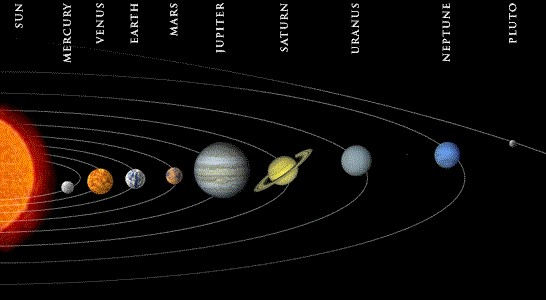
\includegraphics[width=0.6\textwidth]{Solar.jpg}
\caption{Solar System}
\label{fig:SolarSystem}
\end{figure}

% Figure~\ref{fig:SolarSystem}

Those elliptical motions (orbits) can best be figured out by understanding the general equation of planetary motion in the Cartesian co-ordinates system. Let us consider the following figure to best picture our scenario.

\begin{figure}[H]
\centering
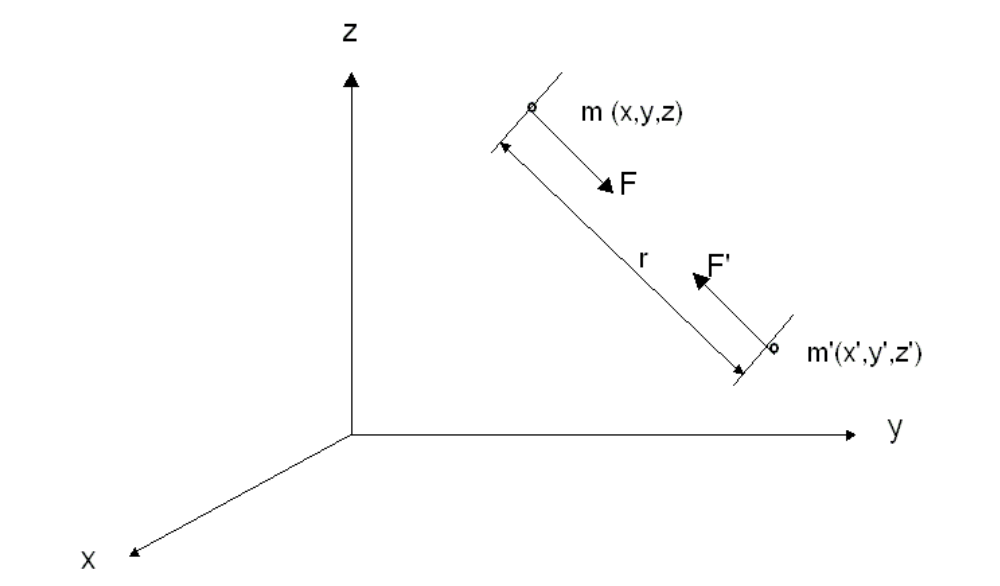
\includegraphics[width=.9\textwidth]{cs.png}
\caption{Representation of two bodies under gravitational attraction in Cartesian co-ordinates}
\label{fig:cs}
\end{figure}


In this project we are going to derive the equations of planetary motion based on the assumption that the masses of the planets can be approximated to point masses. This is reasonable cue to the vast distances between bodies in the solar system.

Then, according to the \textit{Newton's law of gravitational force} acting on each of the masses we obtain the following. 

\[\textbf{F} = G\frac{mm'}{r^2}({\hat{\textbf{r}}})\]
\[\textbf{F'} = G\frac{mm'}{r^2}({-\hat{\textbf{r}}})\]
\\
The respective components F\textsubscript{x}, F\textsubscript{y} and F\textsubscript{z}  of the force \textbf{F}, are: 


\[ F_x = F\frac{x'-x}{r}; \] 
\[ F_y = F\frac{y'-y}{r}; \] 
\[ F_z = F\frac{z'-z}{r}. \]
\\
Furthermore, following \textit{Newton’s second law of dynamics} we obtain:

\[ F_x = m\frac{d^2 x}{dt^2}; \]
\[ F_y = m\frac{d^2 y}{dt^2}; \]
\[ F_z = m\frac{d^2 z}{dt^2}.  \]

\pagebreak

Combining both set of equations, we finally get:

\[ \frac{d^2 x}{dt^2} = Gm'\frac{x'-x}{r^3}; \]
\[ \frac{d^2 y}{dt^2} = Gm'\frac{y'-y}{r^3}; \]
\[ \frac{d^2 z}{dt^2} = Gm'\frac{z'-z}{r^3}. \]

\begin{equation}
\text{Where \textbf{r}, is given by: \space\space\space} r = \sqrt{(x'-x)^2+(y'-y)^2+(z'-z)^2}
\end{equation}

Where $G$ is a gravitational force and $m$ and $M$ are masses of the given planet and Sun respectively, $r$ is the distance between the planet and the Sun and $F$ is the force.

\pagebreak

\section{IVP - Initial Value Problem}
By using the general second order ordinary differential equation system of planetary motion we will now be able to discuss the dynamics of such a motion for all the planets in our solar system including the Sun. In order to reach this realization we designed a global system of equations, accounting for all the interactions of \textit{j} bodies of masses $m_{1},m_{2}...,m_{j}$ on a given body, $\alpha$ of mass $m_{\alpha}$.

Then our system of equation is:\\

$$\dfrac{d^{2}x_{\alpha}}{dt^{2}}=\sum_{j=1;j\neq\alpha}^{nb}Gm_{j}\dfrac{x_{j}-x_{\alpha}}{(r_{j,\alpha})^{3}}$$
$$\dfrac{d^{2}y_{\alpha}}{dt^{2}}=\sum_{j=1;j\neq\alpha}^{nb}Gm_{j}\dfrac{y_{j}-y_{\alpha}}{(r_{j,\alpha})^{3}}$$
$$\dfrac{d^{2}z_{\alpha}}{dt^{2}}=\sum_{j=1;j\neq\alpha}^{nb}Gm_{j}\dfrac{z_{j}-z_{\alpha}}{(r_{j,\alpha})^{3}}$$
$$r_{j,\alpha}=\sqrt[]{(x_{j}-x_{\alpha})^{2}+(y_{j}-y_{\alpha})^{2}+(z_{j}-z_{\alpha})^{2}}$$\\
where,\\
$nb$ - Number of bodies which we consider\\
$G$ - Constant of universal gravitation\\
$m_{j}$ - Mass of body $j$\\
$r_{j,\alpha}$ - Distance between body $j$ and body $\alpha$\\
$x_{\alpha},y_{\alpha},z_{\alpha}$ - Cartesian coordinates of body $\alpha$\\
$x_{j},y_{j},z_{j}$ - Cartesian coordinates of body $j$\\\\
We can convert this system of equations into a standard initial value problem in the following way:\\
$$Y=\begin{bmatrix}
x\\y\\z\\v_{x}\\v_{y}\\v_{z}
\end{bmatrix}=\begin{bmatrix}
x\\y\\z\\\dfrac{dx}{dt}\\\dfrac{dy}{dt}\\\dfrac{dz}{dt}
\end{bmatrix}$$
thus,\\
$$\dfrac{dY}{dt}=F(t,Y)\Rightarrow\dfrac{d}{dt}\begin{bmatrix}
x\\y\\z\\v_{x}\\v_{y}\\v_{z}
\end{bmatrix}=\begin{bmatrix}
v_{x}\\v_{y}\\v_{z}\\\sum_{j=1;j\neq\alpha}^{nb}Gm_{j}\dfrac{x_{j}-x_{\alpha}}{(r_{j,\alpha})^{3}}\\\sum_{j=1;j\neq\alpha}^{nb}Gm_{j}\dfrac{y_{j}-y_{\alpha}}{(r_{j,\alpha})^{3}}\\\sum_{j=1;j\neq\alpha}^{nb}Gm_{j}\dfrac{z_{j}-z_{\alpha}}{(r_{j,\alpha})^{3}}
\end{bmatrix}$$\\
where,\\
$G=6.67E^{-11} m^{3}kg^{1}s^{-2}$  \\
$nb := \text{number of bodies} = 10 $\\

\pagebreak

\begin{landscape}
After converting our $2^{nd}$ order system of ODE's to a $1^{st}$ order system of ODE's, system of equations, we needed a set of initial values for our subsequent ODE Solver. This set of initial states is obtained from the JPL (Jet Propulsion Lab) ephemeris database using the HORIZION web interface. This comprised of the initial states positions (both x y z co-ordinates) and velocities (both x y z co-ordinates), masses and mean radius of all 10 major bodies involved in our solar system.\\

The following table summarizes this initial states corresponding to the solar system configuration on April 6th, 2018:
\\\\\\\\\\\\\\\\
% Table generated by Excel2LaTeX from sheet 'IVP (Sec)'
\begin{table}[htbp]
  \centering
  \caption{Initial States from JPL HORIZONS System}
    \begin{tabular}{|c|l|r|r|r|r|r|r|r|r|}
\cmidrule{3-10}    \multicolumn{1}{r}{} &            & \multicolumn{3}{c|}{\cellcolor[rgb]{ .788,  .788,  .788}\textbf{POSITION (m)}} & \multicolumn{3}{c|}{\cellcolor[rgb]{ .788,  .788,  .788}\textbf{VELOCITY (m/sec)}} & \multicolumn{1}{l|}{\cellcolor[rgb]{ .788,  .788,  .788}\textbf{(kg)}} & \multicolumn{1}{l|}{\cellcolor[rgb]{ .788,  .788,  .788}\textbf{(m)}} \\
    \midrule
    \multicolumn{1}{|l|}{\textbf{\#}} & \textbf{BODY} & \multicolumn{1}{l|}{\textbf{PX}} & \multicolumn{1}{l|}{\textbf{PY}} & \multicolumn{1}{l|}{\textbf{PZ}} & \multicolumn{1}{l|}{\textbf{VX}} & \multicolumn{1}{l|}{\textbf{VY}} & \multicolumn{1}{l|}{\textbf{VZ}} & \multicolumn{1}{l|}{\textbf{MASS}} & \multicolumn{1}{l|}{\textbf{RADIUS}} \\
    \midrule
    \rowcolor[rgb]{ .851,  .882,  .949} 1          & SUN        & 1.81899E+08 & 9.83630E+08 & -1.58778E+07 & -1.12474E+01 & 7.54876E+00 & 2.68723E-01 & 1.98854E+30 & 6.95500E+08 \\
    \midrule
    2          & MERCURY    & -5.67576E+10 & -2.73592E+10 & 2.89173E+09 & 1.16497E+04 & -4.14793E+04 & -4.45952E+03 & 3.30200E+23 & 2.44000E+06 \\
    \midrule
    \rowcolor[rgb]{ .851,  .882,  .949} 3          & VENUS      & 4.28480E+10 & 1.00073E+11 & -1.11872E+09 & -3.22930E+04 & 1.36960E+04 & 2.05091E+03 & 4.86850E+24 & 6.05180E+06 \\
    \midrule
    4          & EARTH      & -1.43778E+11 & -4.00067E+10 & -1.38875E+07 & 7.65151E+03 & -2.87514E+04 & 2.08354E+00 & 5.97219E+24 & 6.37101E+06 \\
    \midrule
    \rowcolor[rgb]{ .851,  .882,  .949} 5          & MARS       & -1.14746E+11 & -1.96294E+11 & -1.32908E+09 & 2.18369E+04 & -1.01132E+04 & -7.47957E+02 & 6.41850E+23 & 3.38990E+06 \\
    \midrule
    6          & JUPITER    & -5.66899E+11 & -5.77495E+11 & 1.50755E+10 & 9.16793E+03 & -8.53244E+03 & -1.69767E+02 & 1.89813E+27 & 6.99110E+07 \\
    \midrule
    \rowcolor[rgb]{ .851,  .882,  .949} 7          & SATURN     & 8.20513E+10 & -1.50241E+12 & 2.28565E+10 & 9.11312E+03 & 4.96372E+02 & -3.71643E+02 & 5.68319E+26 & 5.82320E+07 \\
    \midrule
    8          & URANUS     & 2.62506E+12 & 1.40273E+12 & -2.87982E+10 & -3.25937E+03 & 5.68878E+03 & 6.32569E+01 & 8.68103E+25 & 2.53620E+07 \\
    \midrule
    \rowcolor[rgb]{ .851,  .882,  .949} 9          & NEPTUNE    & 4.30300E+12 & -1.24223E+12 & -7.35857E+10 & 1.47132E+03 & 5.25363E+03 & -1.42701E+02 & 1.02410E+26 & 2.46240E+07 \\
    \midrule
    10          & PLUTO      & 1.65554E+12 & -4.73503E+12 & 2.77962E+10 & 5.24541E+03 & 6.38510E+02 & -1.60709E+03 & 1.30700E+22 & 1.19500E+06 \\
    \bottomrule
    \end{tabular}%
  \label{tab:addlabel}%
\end{table}%
\end{landscape}


\pagebreak

\section{Numerical method description}
Before diving into writing and implementing our own numerical method of ODE Solver we needed to verify our designed IVP model of the solar system by existing and certified ODE solvers such as "ode45" and "ode113". These two solvers amongst many others where chosen for particular reasons we will discuss in the next section.\\

After simulating our IVP with the above solvers, we obtained positive results (discussed in the next section) validating our designed IVP model for the solar system.\\

The next step was to implement from scratch our own ODE solver and apply the designed IVP to it. We made the choice of implementing an \textbf{Explicit Runge-Kutta method (ERK)}. But before we could used this numerical method, we first needed to define our RK-stages $(\nu)$, RK-nodes $(c_{i})$, RK-weights $(b_{i})$ and RK-matrix $(A=[a_{ij}])$. And, verify its order of convergence, exactness and stability.
\\\\The general equations of an ERK is:\\
$$y_{n+1}=y_{n}+h\sum_{j=1}^{\nu}b_{j}f(t_n+c_{j}h,\xi_{j})$$
\\where\\  
\indent$\xi_{1}=y_{n}$\\
\indent$\xi_{2}=y_{n}+ha_{2,1}f(t_{n},\xi_{1})$\\
\indent$\xi_{3}=y_{n}+ha_{3,1}f(t_{n},\xi_{1})+ha_{3,2}f(t_{n}+c_{2}h,\xi_{2})$\\
\indent\;\;\;\;\;\vdots\\
\indent$\xi_{i}=y_{n}+h\sum_{j=1}^{i-1}a_{i,j}f(t_n+c_{j}h,\xi_{j}),\;\;\;\;i=1,\ldots,\nu$\\
\\and $h$ is the step size of our time span. According to our designed IVP, $\xi_{i}$ will be a vector of $6*nb = 6*10=60$ elements. Similarly, $y_{n+1}$ also will be a vector of 60 elements.

\subsection{Definition of our RK method}
The chosen ERK for our implementation has the following parameters:


\[ \nu = 4\\ \]
\[ c = \begin{bmatrix}
	0 & .5 & .5 & 1
\end{bmatrix} \]
\[ b = \begin{bmatrix}
	1/6 & 1/3 & 1/3 & 1/6
\end{bmatrix} \]
\[ A=
  \begin{bmatrix}
    0 & 0 & 0 & 0 \\ 
    .5 & 0 & 0 & 0 \\ 
    0 & .5 & 0 & 0 \\ 
    0 & 0 & 1 & 0
  \end{bmatrix} \]
This method is identified as an Explicit Runge-Kutta method due to its lower triangular matrix, A. Additionally, to the above definition, the $\xi_{i}$'s are as follows:\\
\indent$\xi_{1}=y_{n}$\\
\indent$\xi_{2}=y_{n}+.5hf(t_{n},\xi_{1})=y_{n}+.5hf(t_{n},y_{n})$\\
\indent$\xi_{3}=y_{n}+.5hf(t_{n}+c_{2}h,\xi_{2})=y_{n}+.5hf\Big(t_{n}+.5h,y_{n}+.5hf(t_{n},y_{n})\Big)$\\
\indent$\xi_{4}=y_{n}+hf(t_{n}+c_{3}h,\xi_{3})=y_{n}+hf\Big(t_{n}+.5h,y_{n}+.5hf\Big(t_{n}+.5h,y_{n}+.5hf(t_{n},y_{n})\Big)\Big)$\\\\
By applying these $\xi_{i}$'s on the general ERK formula, we can predict order of convergence of this method.


\subsection{Order of convergence of the chosen RK}
The chosen ERK method defined in the previous subsection is of stage, $\nu=4$ and thus of order 4. This claim can further be verified by applying the ERK on the following IVP; applied under different values of the step size and interpreting the resultant graphs.\\

IVP: \space $y'(t)=-y$; \space $y_{0}=1$ when $t=0$\\

The ERK will by applied with step sizes: $h=.1/2^k$, \space with $k=1,2,3,4. $ \\

The exact solution for this IVP is known to be: $y(t)=e^{-t}$ \\

After running the written MatLab codes for this text, the following graphs were obtained:

\begin{figure}[!ht]
\centering
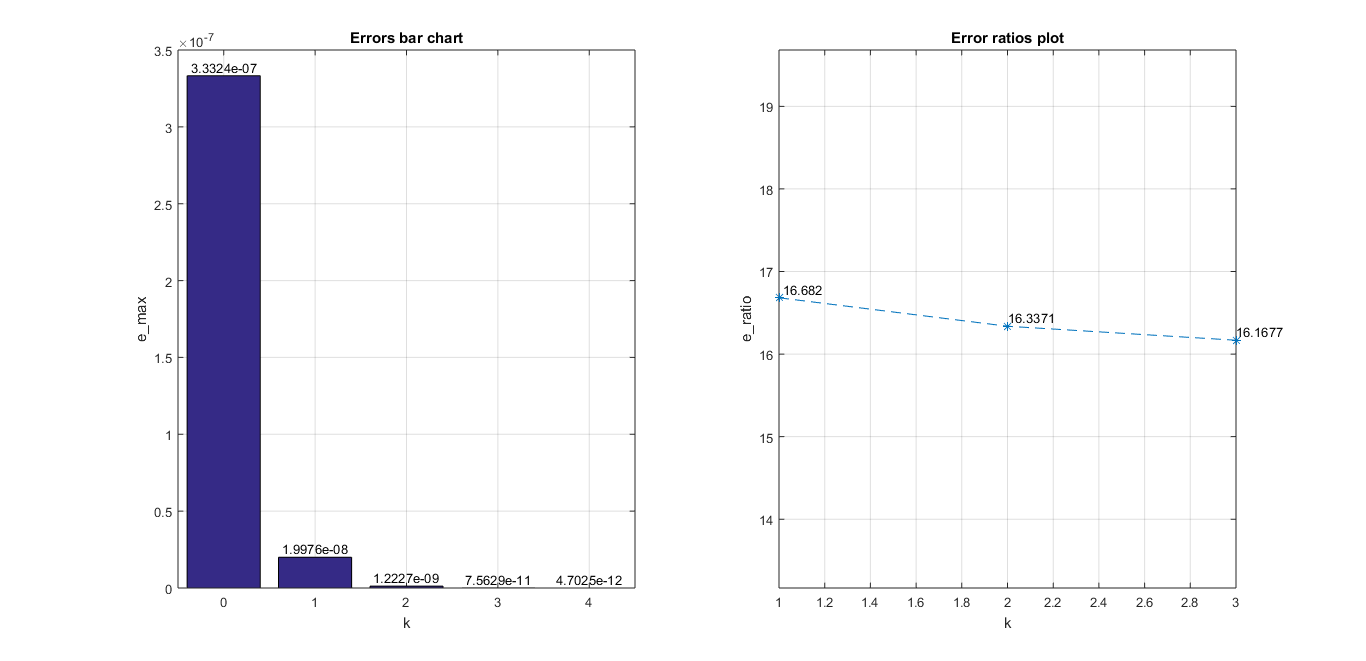
\includegraphics[width=1\textwidth]{testeer.png}
\caption{Error/Error-ratio test}
\label{fig:testeer}
\end{figure}

By inspecting the error-ratio plot on the right of the above figure we observe a trend:  $$\textrm{error-ratio}\rightarrow 16 = 2^4 = 2^p$$

This interpretation let us conclude that the order of convergence, $p=4$.\\\\
According to the definition of exactness, a given method is exact for the polynomials of degree less than or equal to $d$ , where $d$ is the degree of the exactness and usually it is equal to the order of the method. Therefore, the chosen ERK method is exact for the polynomials of degree less than or equal to 4. Because, 4 is the order of convergence of this ERK method.

Additionally, it can be interpreted from the errors bar chart that the ERK method of oder 4 is exact, as the error is in a close neighborhood of zero. 

\subsection{verification of stability of the chosen RK}
The stability of RK method can be define according to the general equation of RK and the following equations. Then apply RK method for the following IVP.\\
$$y'=\lambda y$$
$$y(t_{0})=y_{0}$$
Now consider the equations for the $\xi$'s. In general its given by:\\
$$\xi_{k}=y_{n}+h\lambda\sum_{i=1}^{k}a_{k,i}f(t_n+c_{i}h,\xi_{i})$$\\
In this equation, $\sum_{i=1}^{k}a_{k,i}f(t_n+c_{i}h,\xi_{i})$ is a dot product of the $k^{th}$ row of the matrix $A$ and a vector of $\xi$. Let's define some vectors as follows,\\
$$\xi=\begin{bmatrix}
\xi_{1}\\\xi_{2}\\\vdots\\\xi_{\nu}
\end{bmatrix},\;\; b=\begin{bmatrix}
b_{1}\\b_{2}\\\vdots\\b_{\nu}
\end{bmatrix},\;\;\textbf{1}=\begin{bmatrix}
1\\1\\\vdots\\1
\end{bmatrix}$$
Then, the system of equations for $\xi$'s can be represented as;
$$\xi=y_{n}.\textbf{1}+h\lambda A\xi\Rightarrow \xi=(I-h\lambda A)^{-1}.\textbf{1}.y_{n}$$ 
By using this $\xi$ in the general equation of RK, we can be obtain,
$$y_{n}=(1+zb^{T}(I-zA)^{-1}\textbf{1})^{n}y_{0}\;\;\;where\;\;z=h\lambda$$
Then the stability domain of RK can be find when $\left|r(z)\right|<1$ where $r(z)=1+zb^{T}(I-zA)^{-1}\textbf{1}$.\\\\
By using above condition, can be find the stability domain of the chosen ERK, which is mentioned in subsection $(3.1)$. Therefore,\\\\
$I-zA=
  \begin{bmatrix}
    1 & 0 & 0 & 0 \\ 
    -.5z & 1 & 0 & 0 \\ 
    0 & -.5z & 1 & 0 \\ 
    0 & 0 & -z & 1
  \end{bmatrix} $ and $(I-zA)^{-1}=
  \begin{bmatrix}
    1 & 0 & 0 & 0 \\ 
    .5z & 1 & 0 & 0 \\ 
    .25z^{2} & .5z & 1 & 0 \\ 
    .25z^{3} & .5z^{2} & z & 1
  \end{bmatrix} $\\\\\\
  $b^{T}(I-zA)^{-1}\textbf{1}=\begin{bmatrix}
  1/6 & 1/3 & 1/3 & 1/6
  \end{bmatrix}\begin{bmatrix}
    1 & 0 & 0 & 0 \\ 
    .5z & 1 & 0 & 0 \\ 
    .25z^{2} & .5z & 1 & 0 \\ 
    .25z^{3} & .5z^{2} & z & 1
  \end{bmatrix}\begin{bmatrix}
  1 \\ 1 \\ 1 \\ 1
  \end{bmatrix}=1+\dfrac{z}{2}+\dfrac{z^{2}}{6}+\dfrac{z^{3}}{24}$\\\\
  $\Rightarrow r(z)=1+z\Big(1+\dfrac{z}{2}+\dfrac{z^{2}}{6}+\dfrac{z^{3}}{24}\Big)=1+z+\dfrac{z^{2}}{2}+\dfrac{z^{3}}{6}+\dfrac{z^{4}}{24}$\\\\
  By using Mathematica codes for $r(z)$, the following stability (shaded) region was obtained:\\
  
\begin{figure}[!ht]
\centering
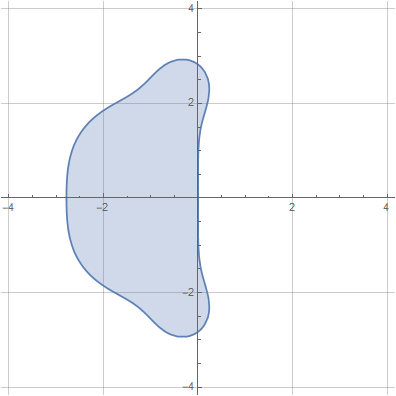
\includegraphics[width=0.5\textwidth]{StabilityDomain.png}
\caption{Stability domain}
\label{fig:stability_domain}
\end{figure}  

According to this stability region it can be concluded that, the chosen ERK method is not A-stable. Because, for a method to be A-stable it must include $\mathbb{C}^{-}$ in its stability region. Despite the fact that an 
A-stability wasn't reached, necessary stability domain could be achieved. This achieved stability will be useful the next section.

\pagebreak

\section{Numerical Results and Discussion}
After a repeated set of simulations we made some adjustments regarding the number of planets considered and the step size to use with the different ODE Solvers.\\

The adjustment made on the number of planet consider, dealt with the non-consideration of planet Pluto. This adjustment was made in order to reduce the computational intensity of our code and enhanced faster calculations.\\

The second adjustment made on the step size, mainly had to constrain the step size to a value of 1. This adjustment was done to obtain better stability with our set of non-stiff ODE Solvers. Mainly, due to the fact that our IVP is a Stiff IVP, and, thereby necessitated (for more appropriate circumstances) a stiff ODE Solver with an A-stability region.\\

Nonetheless, with the appropriate adjustments, the following satisfactory results were obtained and interpreted as follows: \\


\subsection{\textit{Build-in ode45}}

The first ODE used was the ode45. This build-in MatLab ODE Solver was chosen to test the IVP model and make sure it is designed correctly. The result obtained, Fig~\ref{fig:Solar_System_-_ode45}, showed great instability of this ODE Solver due to the stiffness of the IVP. And, the added adjustment couldn't lead to better results.

\begin{figure}[H]
\centering
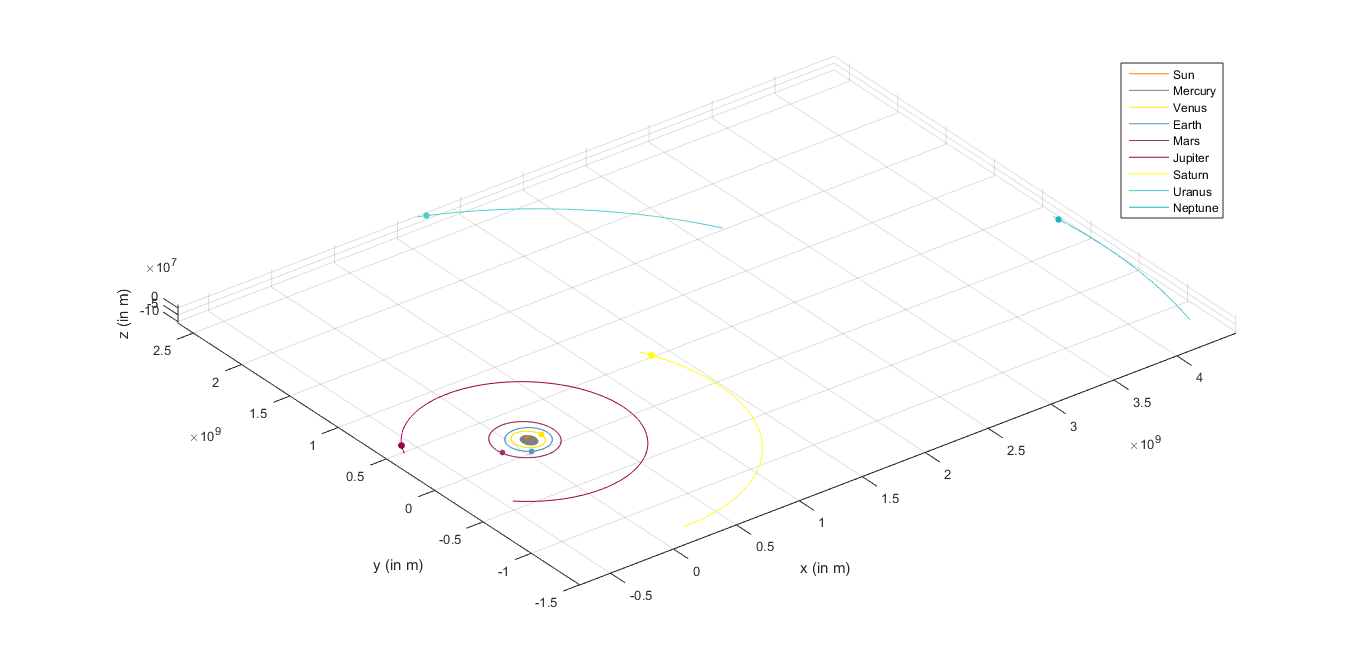
\includegraphics[width=1\textwidth]{Solar_System_-_ode45.png}
\caption{Solar System Simulation - ode45}
\label{fig:Solar_System_-_ode45}
\end{figure}

In the next figure, Fig~\ref{fig:Solar_System_-_ode45_-_ipsim}, we can observe the instability as the parameters of Mercury tend to decay much faster than that of the other planets. This behavior generated an error caused by the lack of better accuracy.

\begin{figure}[H]
\centering
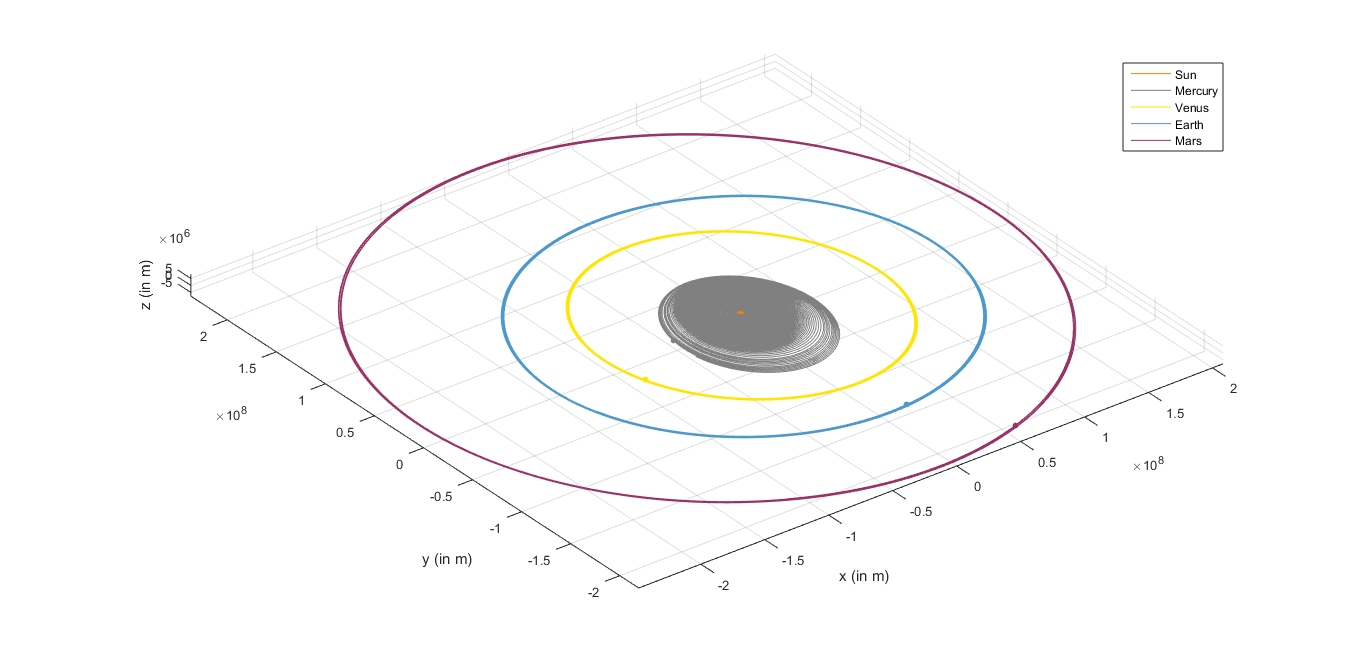
\includegraphics[width=1\textwidth]{Solar_System_-_ode45_-_ipsim.png}
\caption{Solar System Simulation - ode45 - Inner planets }
\label{fig:Solar_System_-_ode45_-_ipsim}
\end{figure}

This ODE Solver couldn't complete the solution and crashed. The following figures show the plot of the distance from the different bodies to the reference point which in this case is not the sun but the origin. 

\begin{figure}[H]
\centering
\begin{subfigure}{.5\textwidth}
\centering
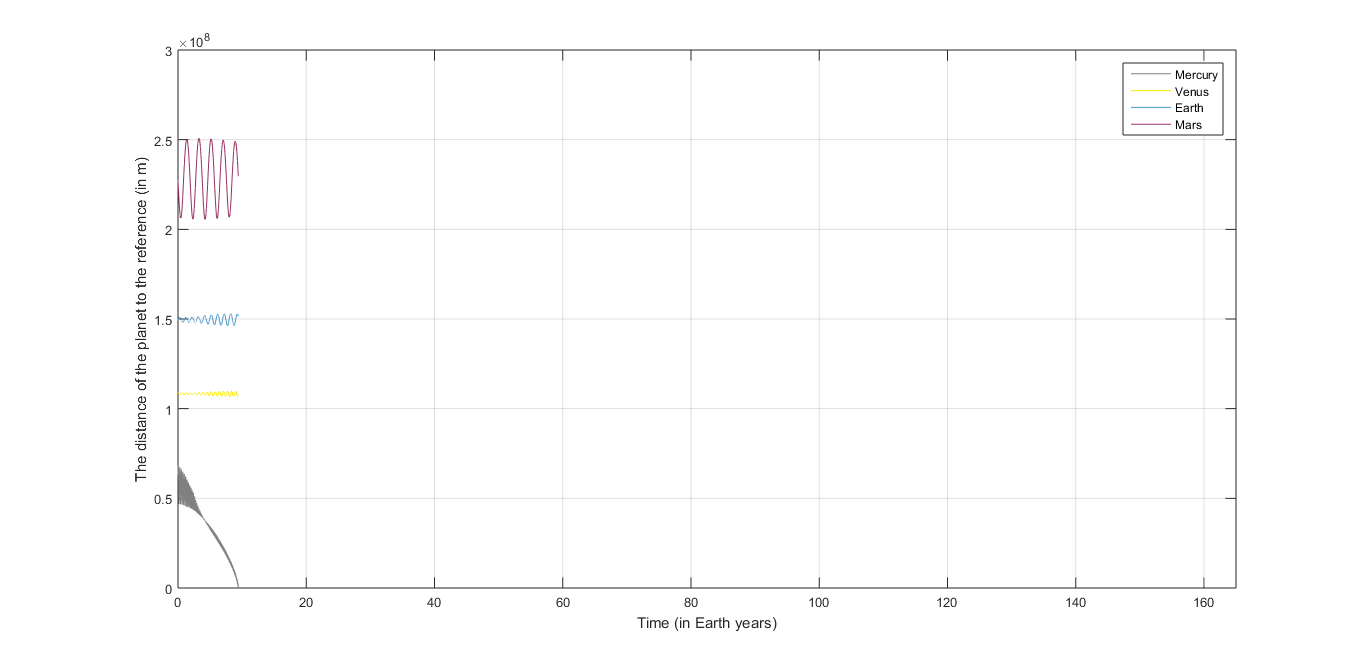
\includegraphics[width=1\textwidth]{Solar_System_-_ode45_-_ip.png}
\caption{Distance from origin - ode45 - Inner planet}
\label{fig:Solar_System_-_ode45_-_ip}
\end{subfigure}%
\begin{subfigure}{.5\textwidth}
\centering
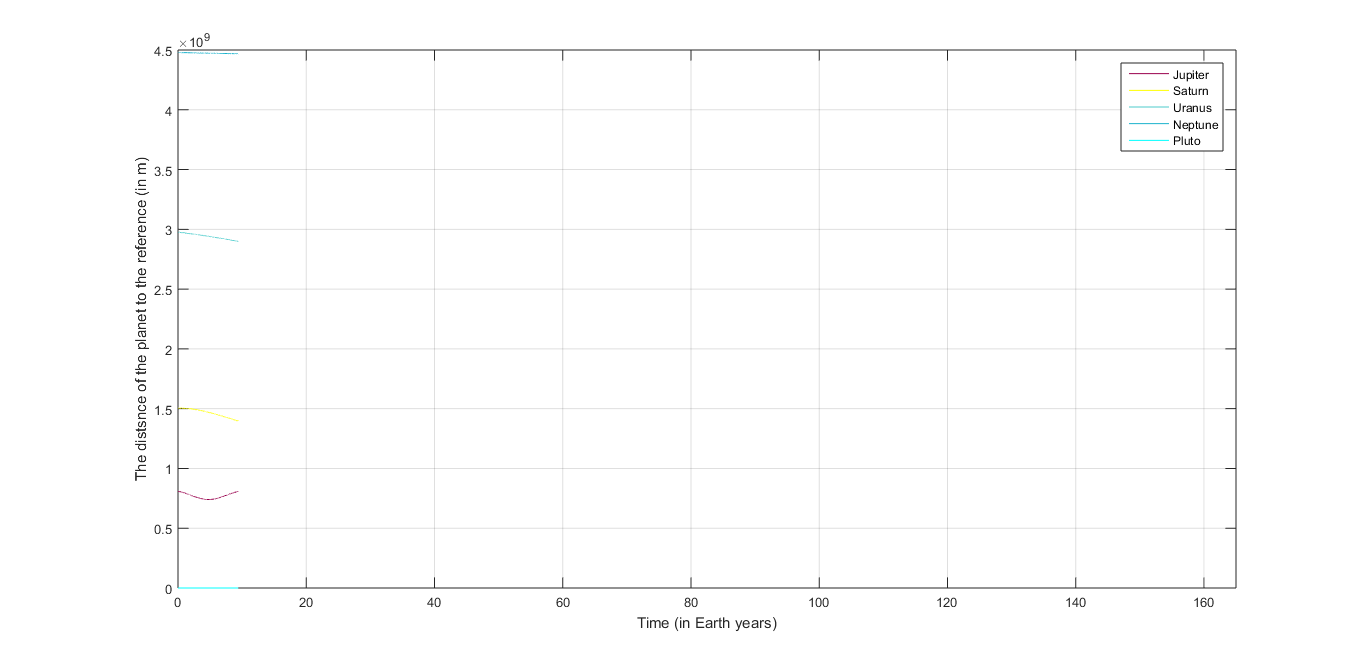
\includegraphics[width=1\textwidth]{Solar_System_-_ode45_-_op.png}
\caption{Distance from origin - ode45 - Outer planet}
\label{fig:Solar_System_-_ode45_-_op}
\end{subfigure}
\begin{subfigure}{.7\textwidth}
\centering
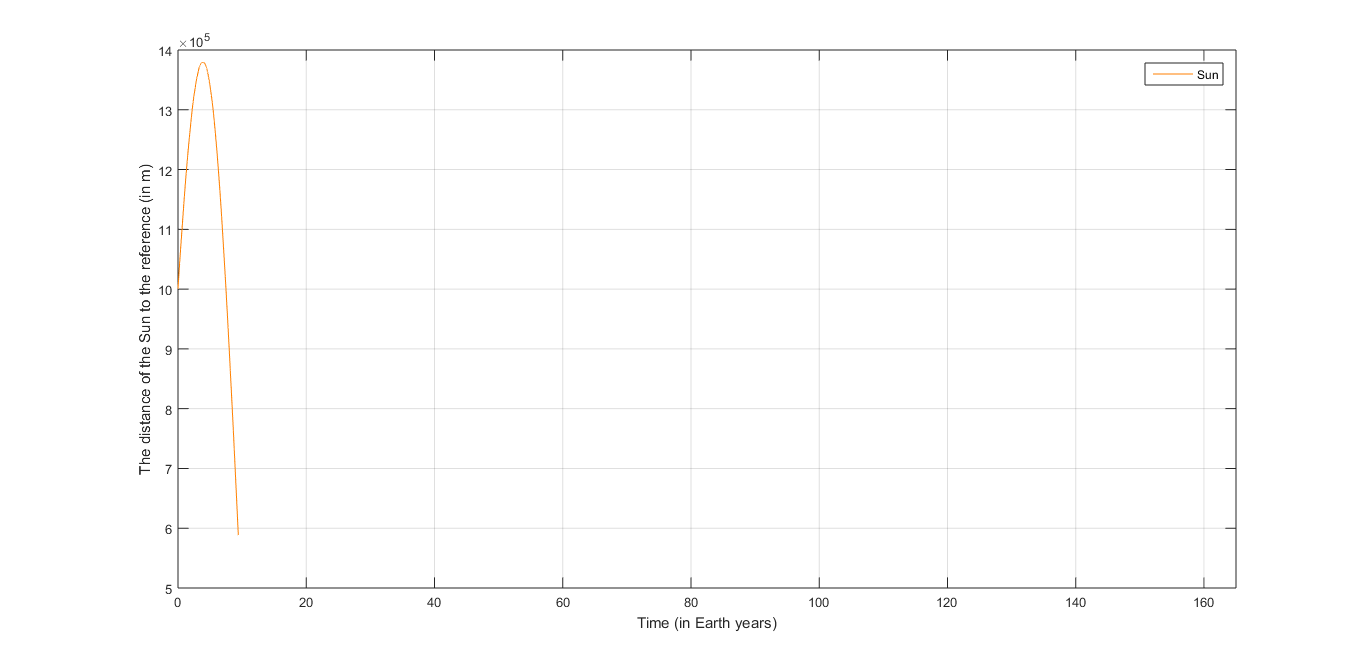
\includegraphics[width=1\textwidth]{Solar_System_-_ode45_-_sun.png}
\caption{Distance from origin - ode45 - Sun}
\label{fig:Solar_System_-_ode45_-_sun}
\end{subfigure} 
\caption{Distance from origin}
\label{fig:Solar_System_-_ode45_-_all}
\end{figure} 

\pagebreak

\subsection{\textit{Build-in ode113}}
By observing from the previous method that the modeled IVP had stringent error tolerances, it was necessary to retry the test of the IVP with higher accuracy ODE Solver as ode113. The ode113 is also a MatLab build-in Solver. The figure, Fig~\ref{fig:Solar_System_-_ode113}, depicts the result obtained.

\begin{figure}[H]
\centering
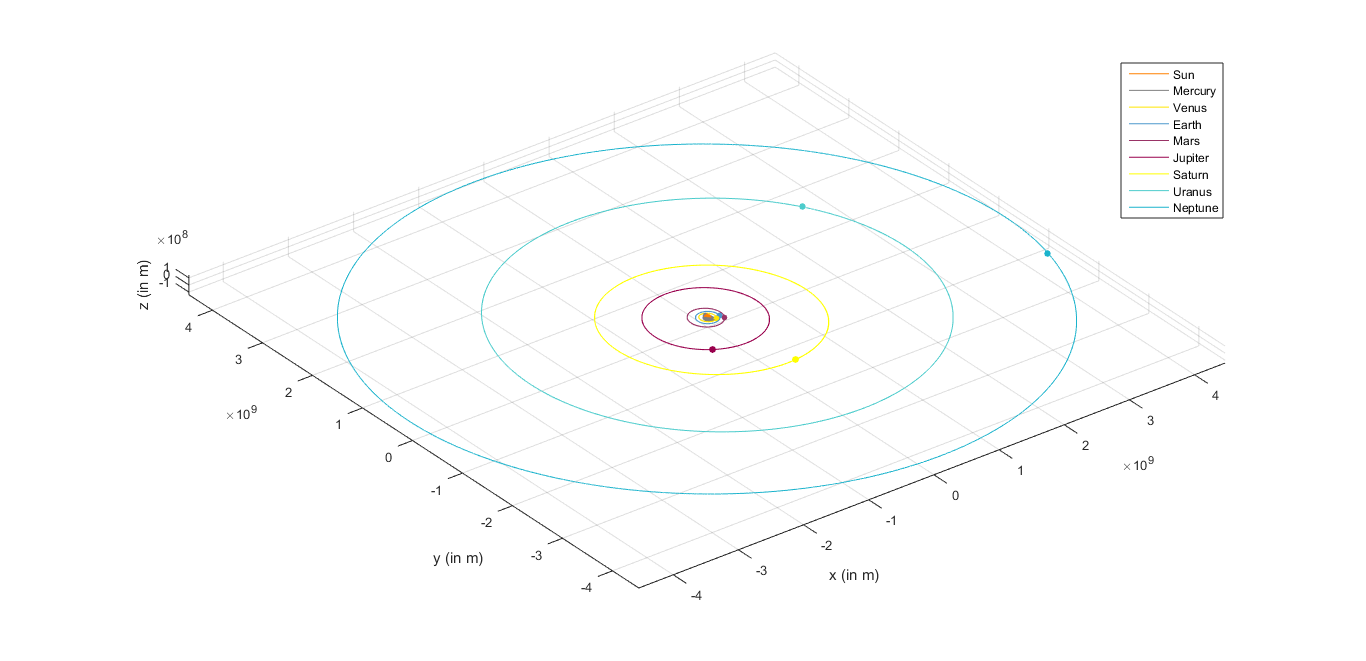
\includegraphics[width=1\textwidth]{Solar_System_-_ode113.png}
\caption{Solar System Simulation - ode113}
\label{fig:Solar_System_-_ode113}
\end{figure}

This result had better stability and calculated a complete solution for a time span corresponding to the period of revolution of the planet Neptune (165 earth years). The result lead to a validation of the IVP model.

\begin{figure}[H]
\centering
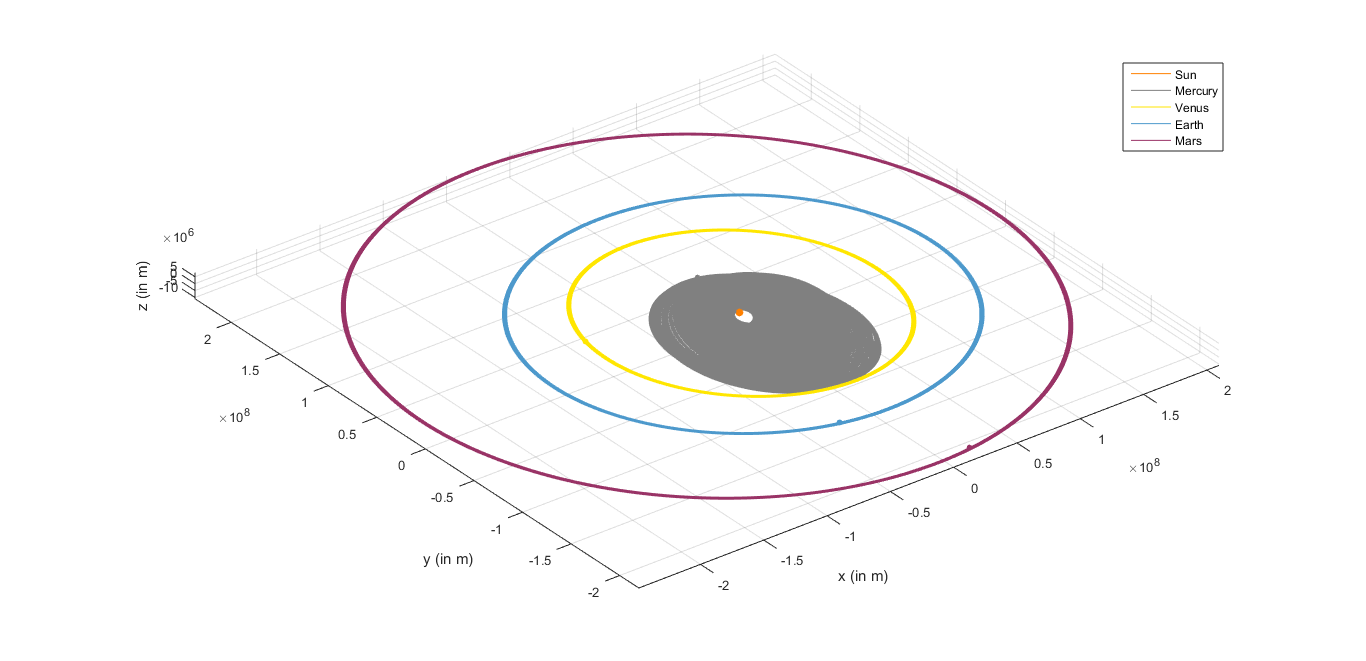
\includegraphics[width=1\textwidth]{Solar_System_-_ode113_-_ipsim.png}
\caption{Solar System Simulation - ode113 - Inner planets }
\label{fig:Solar_System_-_ode113_-_ipsim}
\end{figure}

\begin{figure}[H]
\centering
\begin{subfigure}{.5\textwidth}
\centering
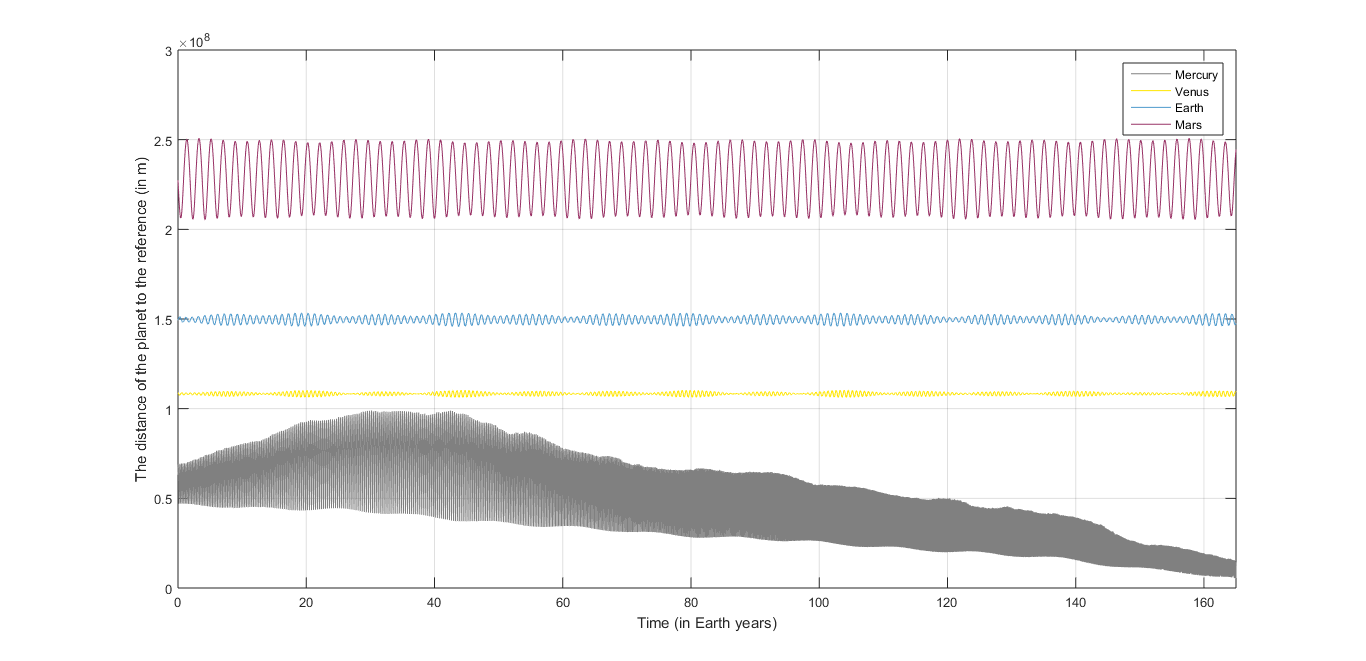
\includegraphics[width=1\textwidth]{Solar_System_-_ode113_-_ip.png}
\caption{Distance from origin - ode113 - Inner planet}
\label{fig:Solar_System_-_ode113_-_ip}
\end{subfigure}%
\begin{subfigure}{.5\textwidth}
\centering
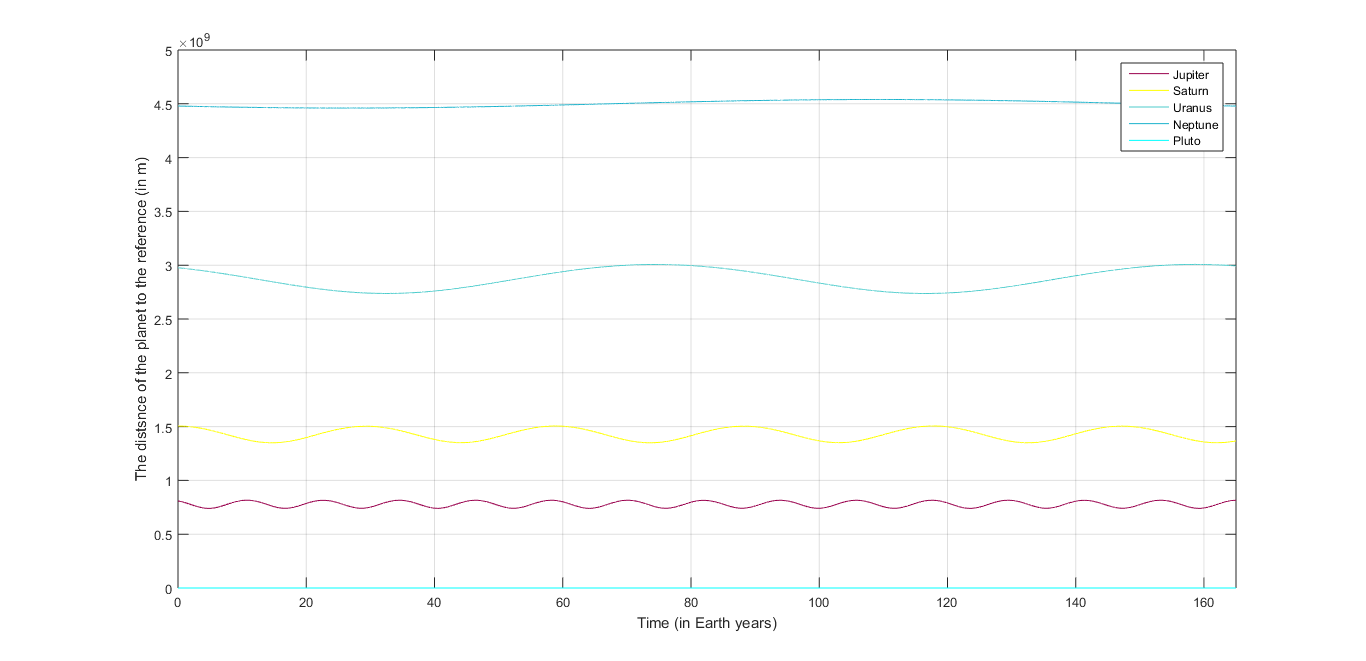
\includegraphics[width=1\textwidth]{Solar_System_-_ode113_-_op.png}
\caption{Distance from origin - ode113 - Outer planet}
\label{fig:Solar_System_-_ode113_-_op}
\end{subfigure}
\begin{subfigure}{.7\textwidth}
\centering
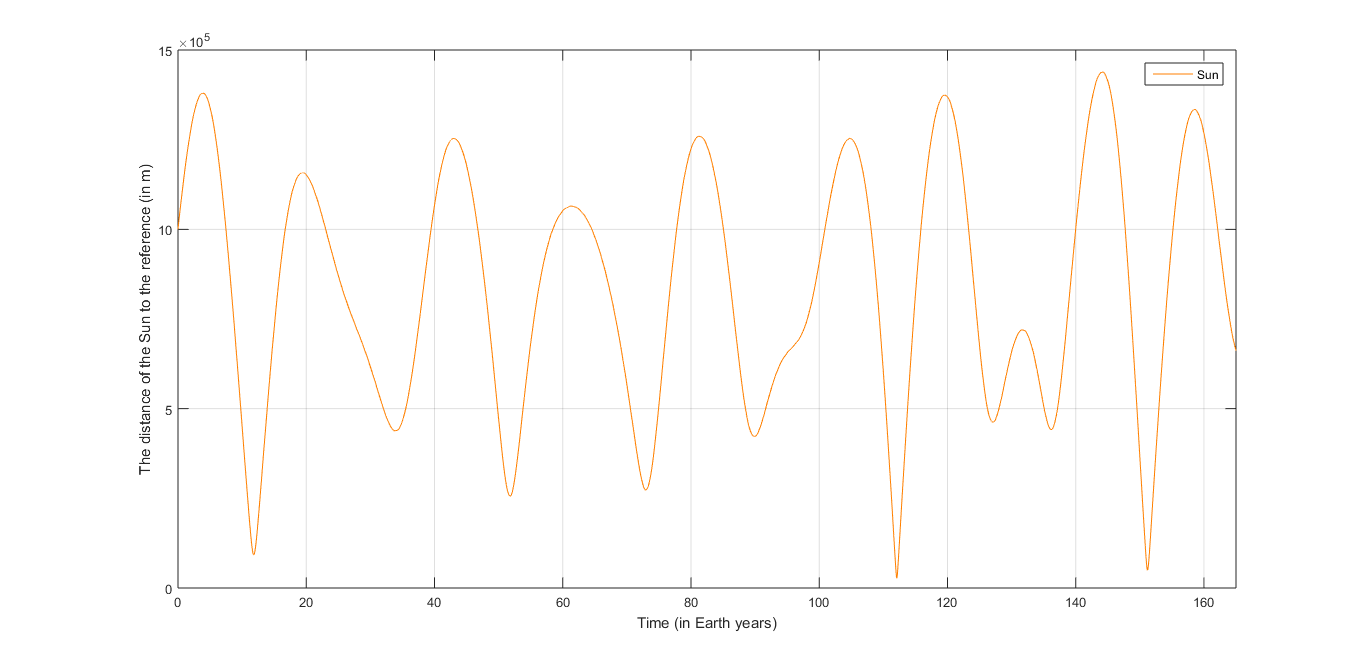
\includegraphics[width=1\textwidth]{Solar_System_-_ode113_-_sun.png}
\caption{Distance from origin - ode113 - Sun}
\label{fig:Solar_System_-_ode113_-_sun}
\end{subfigure} 
\caption{Distance from origin}
\label{fig:Solar_System_-_ode113_-_all}
\end{figure} 



\subsection{\textit{Implemented ERK of order 4, ode652}}
The final step was to build from scratch an ODE Solver to attain better (or similar) results as those obtained with  ode113.\\

The ODE Solver, ode652, coded on MatLab implemented the ERK of order 4 earlier described in the Numerical method section of this paper. This implementation achieved better stability compared to ode113 and ode45. A complete simulation of a time span equivalent to the period of the planet Neptune was obtained. Fig~\ref{fig:Solar_System_-_ode652}, shows this result and Fig~\ref{fig:Solar_System_-_ode652_-_ipsim}, shows a bigger scale of the inner planets of the solar system.

\begin{figure}[H]
\centering
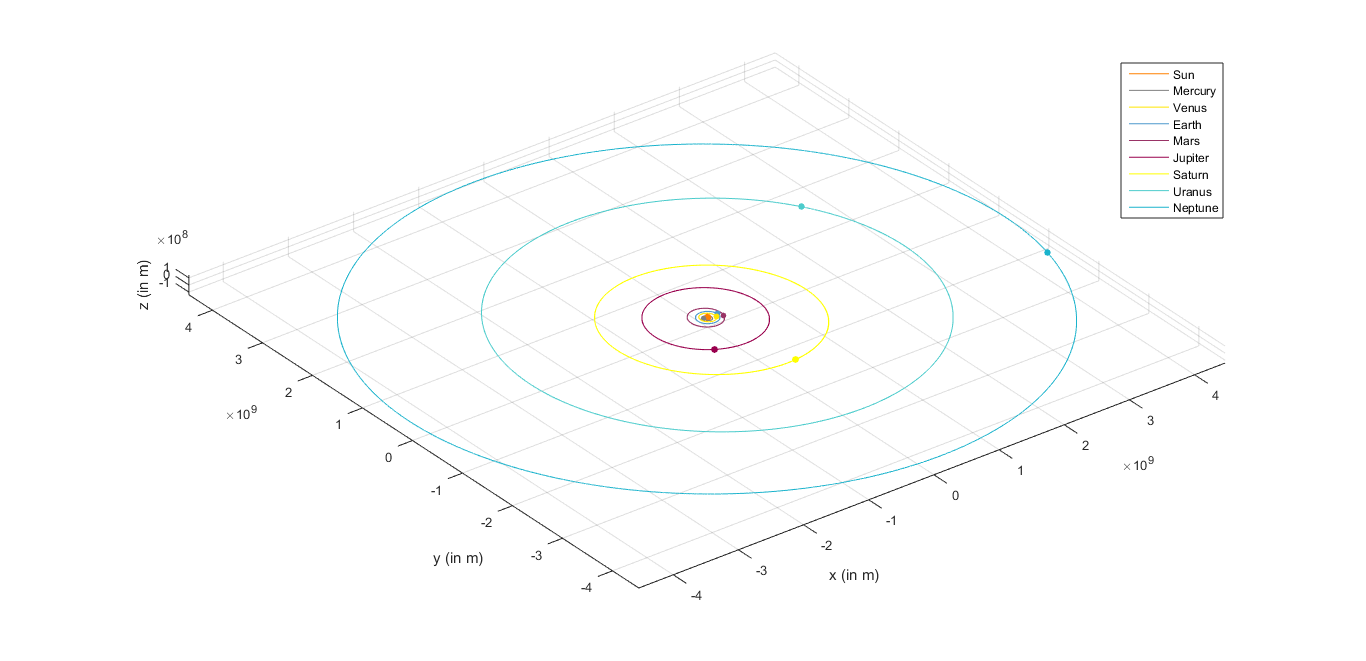
\includegraphics[width=1\textwidth]{Solar_System_-_ode652.png}
\caption{Solar System Simulation - ode652}
\label{fig:Solar_System_-_ode652}
\end{figure}

\begin{figure}[H]
\centering
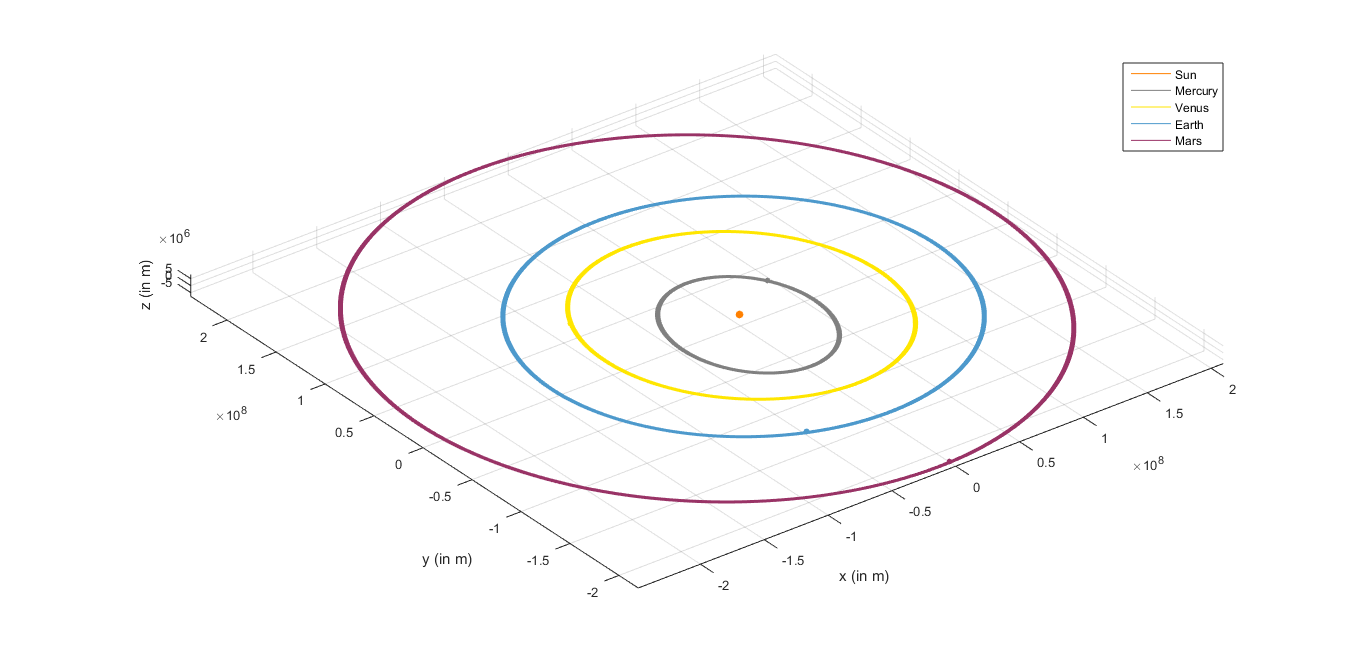
\includegraphics[width=1\textwidth]{Solar_System_-_ode652_-_ipsim.png}
\caption{Solar System Simulation - ode652 - Inner planets }
\label{fig:Solar_System_-_ode652_-_ipsim}
\end{figure}

The above figure and of the distances from the reference point below, clearly shows a more stable revolution of Mercury. This result is obtained by a solution made with better accuracy compared to those of ode113 and ode45.

\begin{figure}[H]
\centering
\begin{subfigure}{.5\textwidth}
\centering
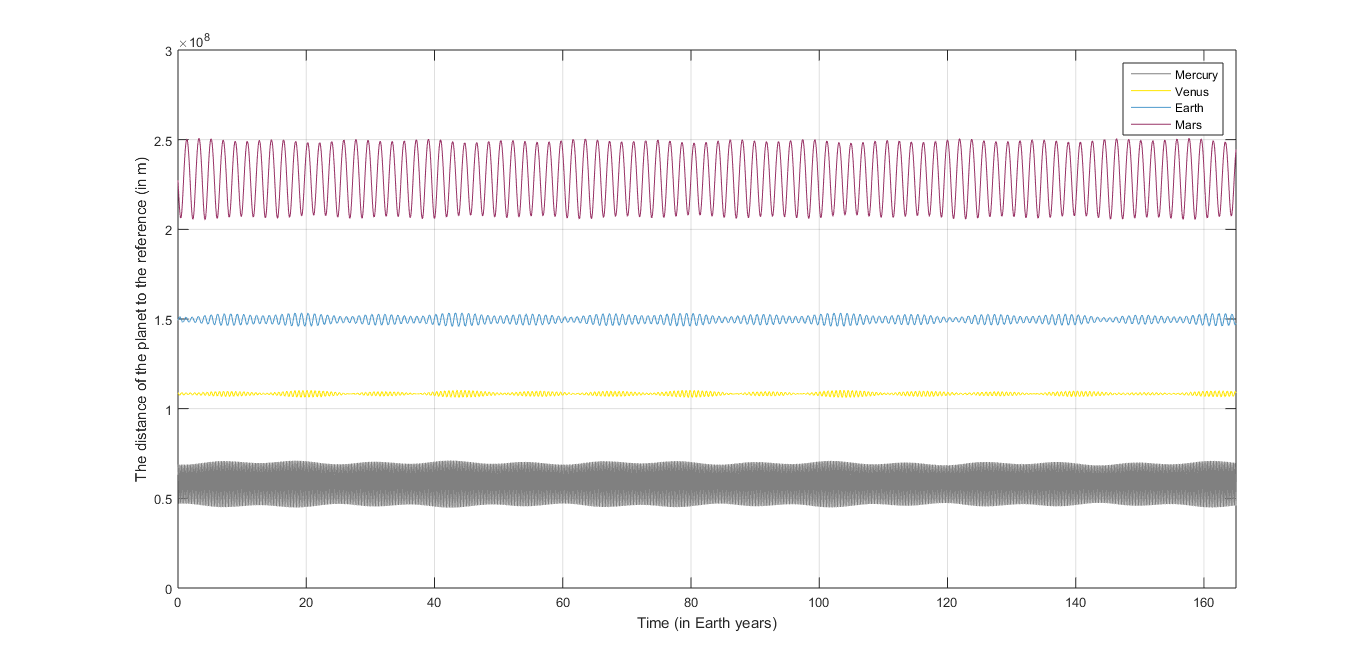
\includegraphics[width=1\textwidth]{Solar_System_-_ode652_-_ip.png}
\caption{Distance from origin - ode652 - Inner planet}
\label{fig:Solar_System_-_ode652_-_ip}
\end{subfigure}%
\begin{subfigure}{.5\textwidth}
\centering
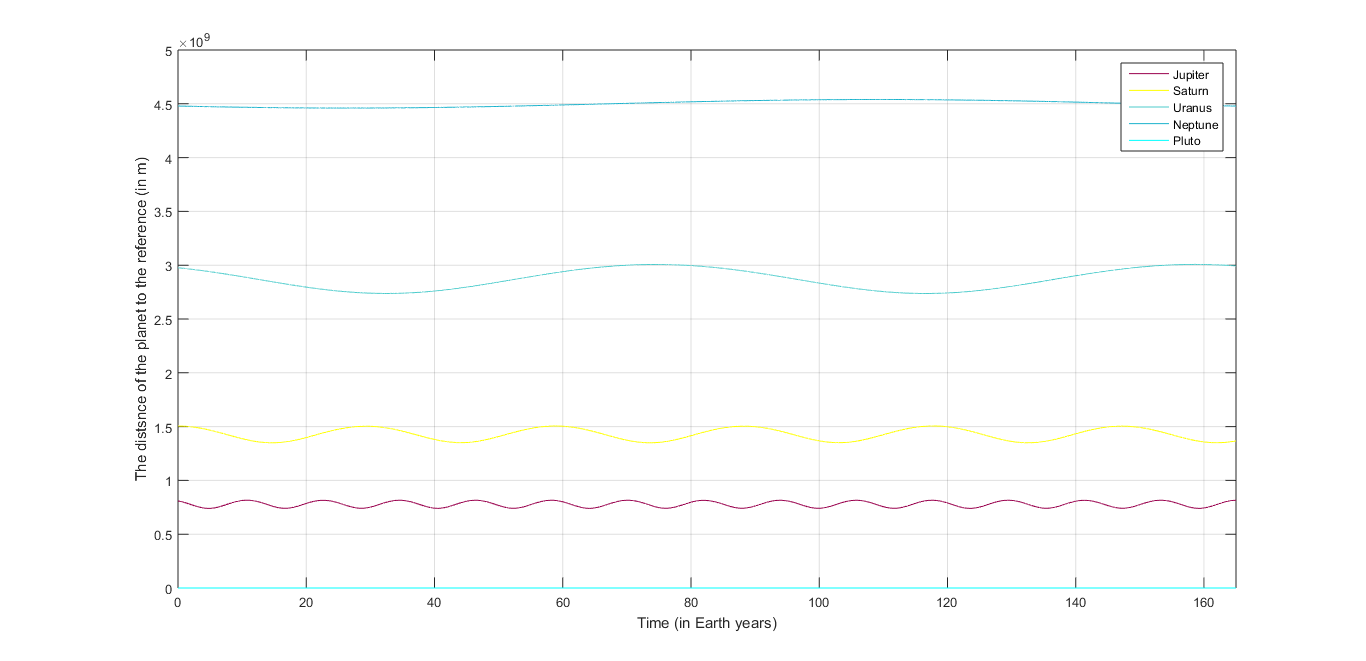
\includegraphics[width=1\textwidth]{Solar_System_-_ode652_-_op.png}
\caption{Distance from origin - ode652 - Outer planet}
\label{fig:Solar_System_-_ode652_-_op}
\end{subfigure}
\begin{subfigure}{.7\textwidth}
\centering
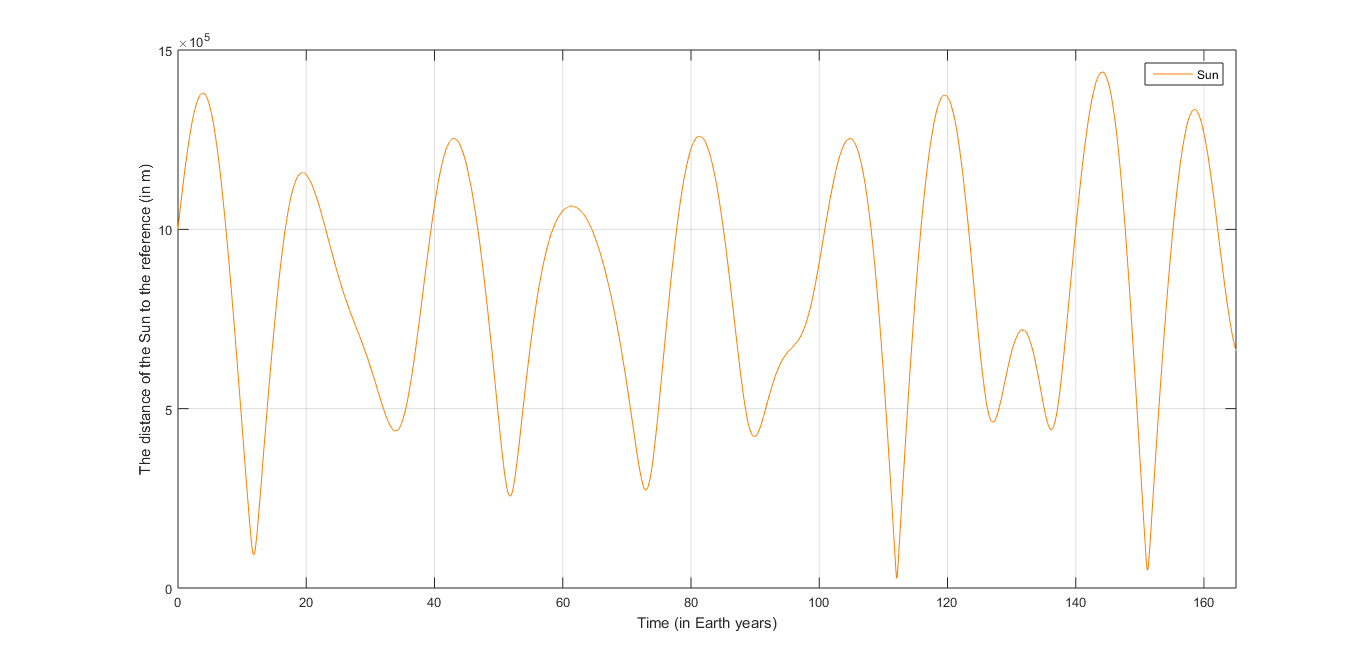
\includegraphics[width=1\textwidth]{Solar_System_-_ode652_-_sun.png}
\caption{Distance from origin - ode652 - Sun}
\label{fig:Solar_System_-_ode652_-_sun}
\end{subfigure} 
\caption{Distance from origin}
\label{fig:Solar_System_-_ode652_-_all}
\end{figure} 

With this implementation the stability domain portrait by the chosen ERK of order 4, showed to sufficient (under certain adjustments) for the obtained solution. 

\pagebreak

\section{Conclusion}
As a summary, the implemented method discussed in this paper is a non A-stable method. Nonetheless, this method had a stability region necessary and sufficient for our implementation. The modeled IVP mentioned under section 2 was analyzed to be stiff due to the existence of some its parameters who tend to grow faster than others (Mercury's). Thereby, higher stability needed to be reached for satisfactory result.\\

After, attempting solutions of the IVP with build-in MatLab ODE Solvers, we realized a very high error dependency of the IVP model. Due to this condition, the choice of implementing the ERK of order 4 was made appropriate because of the better accuracy/stability it provided under certain adjustments.\\

Finally, we were able to implement a method, ode652, with much more better stability than certain build-in MatLab methods, ode45 and ode113 of quite similar non A-stability behavior, to solve the modeled IVP of solar system dynamics.\\ 

\pagebreak

\lstset{language=Matlab,%
    %basicstyle=\color{red},
    breaklines=true,%
    morekeywords={matlab2tikz},
    keywordstyle=\color{blue},%
    morekeywords=[2]{1}, keywordstyle=[2]{\color{black}},
    identifierstyle=\color{black},%
    stringstyle=\color{mylilas},
    commentstyle=\color{mygreen},%
    showstringspaces=false,%without this there will be a symbol in the places where there is a space
    numbers=left,%
    numberstyle={\tiny \color{black}},% size of the numbers
    numbersep=9pt, % this defines how far the numbers are from the text
    emph=[1]{for,end,break},emphstyle=[1]\color{red}, %some words to emphasise
    %emph=[2]{word1,word2}, emphstyle=[2]{style},    
}

\pagebreak

\begin{thebibliography}{9}

\bibitem{latexcompanion} 
ARIEH ISERLES, University of Cambridge, (1992), 
A First Course in the Numerical Analysis
of Differential Equations

\bibitem{NAZA} 
NAZA, (2018), HORIZONS Web-Interface,
\\\url{https://ssd.jpl.nasa.gov/horizons.cgi#top}

\bibitem{InfoPlease} 
InfoPlease, (2018), Basic Planetary Data,
\\\url{https://www.infoplease.com/science-health/solar-system/basic-planetary-data}

\bibitem{MATLAB} 
MATLAB, (2018), Choose an ODE Solver - MATLAB and Simulink,
\\\url{https://www.mathworks.com/help/matlab/math/choose-an-ode-solver.html}

\bibitem{Wikipedia1} 
Wikipedia, (25 October 2017), List of Runge–Kutta methods,
\\\url{https://en.wikipedia.org/wiki/List_of_Runge%E2%80%93Kutta_methods}

\bibitem{Guido} 
Guido Kanschat, (May 2, 2018), Numerical Analysis of Ordinary Differential Equations,
\\\url{https://en.wikipedia.org/wiki/List_of_Runge%E2%80%93Kutta_methods}

\bibitem{Kyriacos} 
Kyriacos Papadatos, (Unknown), THE EQUATIONS OF PLANETARY MOTION AND THEIR SOLUTION,
\\\url{http://gsjournal.net/Science-Journals/Research%20Papers-Astrophysics/Download/3763}

% \bibitem{Wikipedia1} 
% Author, (Date), Title,
% \\\url{url}

\end{thebibliography}

\pagebreak

\begin{appendices}
\lstinputlisting{codes/ode652.m}
\end{appendices}

\end{document}